\chapter{Предисловие}

Если вдруг кто-то не знает, о чем идёт речь - в 70-м году случился первый (без учета полумифических вьетнамских) с окончания корейской войны полноценный воздушный бой с участием советских летчиков. Он-же на долгое время стал последним.

Тащемта, через пару - тройку недель я доделаю большую статью об этом примечательном событии с кучей интервью и карт. А пока - несколько тезисов, которые вылезли в процессе подготовки материала:

0) Никакого боя "20 мигов против 24 миражей" не было. Было несколько отдельных боёв, разнесенных во времени (на минуты) и пространстве (на километры), не больше чем 4 на 8.

\begin{figure}[h!tb] 
	\centering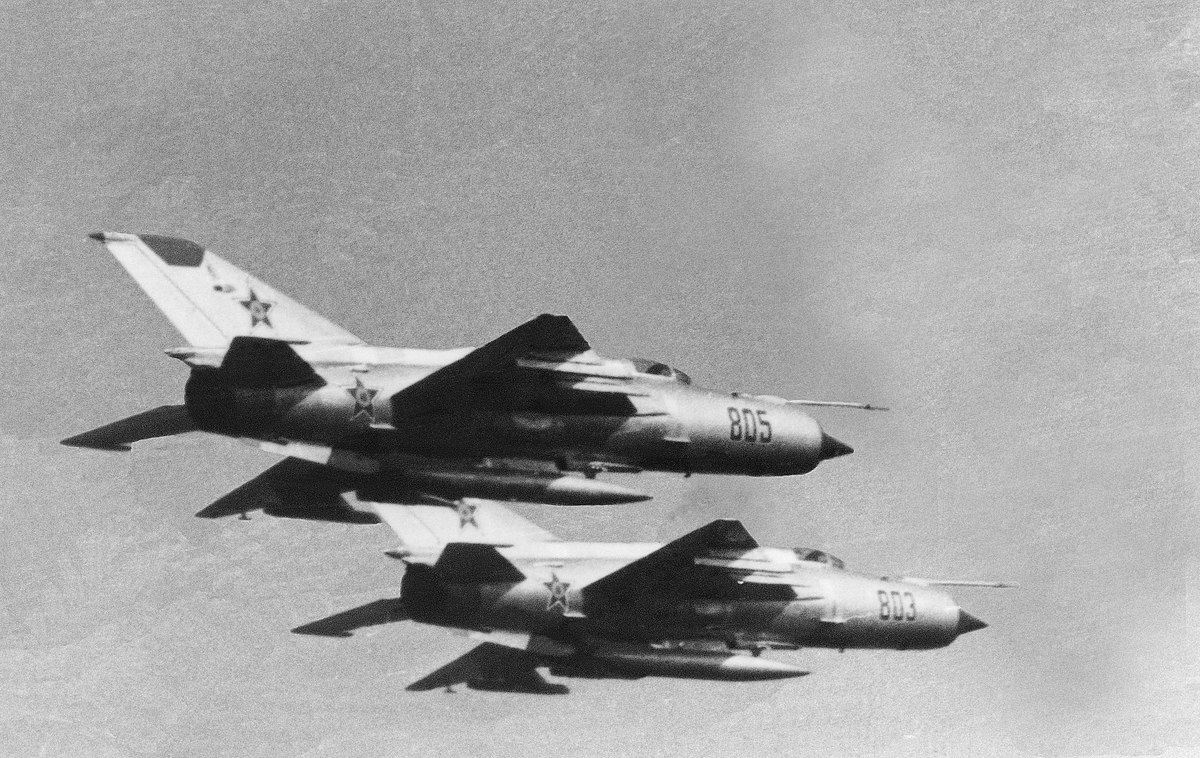
\includegraphics[scale=0.4]{Dolina_0/fY6zrQ81LqI.jpg}
	%	\label{fig:scipion} % Unique label used for referencing the figure in-text\end{document}
	%	%\addcontentsline{toc}{figure}{Figure \ref{fig:placeholder}} % Uncomment to add the figure to the table of contents%----------------------------------------------------------------------------------------
	\caption{Румынские МиГ-21МФ идентичные натуральному}%	CHAPTER 2
\end{figure}
1) Отправляя 2 эскадрильи (окей, эскадрилью и авиаполк) в Египет, в СССР крайне туманно представляли, с кем им предстоит столкнуться. Знали, что "с той стороны" хорошие лётчики. Собственным пилотам вместо реально стоящей информации транслировали набор пропагандистских штампов (про наёмников из США, американские тактики и "элитную" 101-ю эскадрилью и прочее прочее). В целом, израильская завеса параноидальной секретности работала.

2) Советские лётчики не вполне понимали, что летят на полноценную войну. Где иногда убивают. Ну, разумом, может, понимали. Но не сердцем. ИМХО, с этим знанием погибших в том бою было бы меньше.

3) Советская тактика опиралась на Вьетнам (в лучшем случае) или опыт Великой Отечественной (в худшем), и очень сильно привязывала пилота к командам с земли. Как только связь с КП по каким-то причинам прерывалась (например, помехами) - начиналось замешательство. Израильские тактики и опыт египтян изучались , но только в инициативном порядке и "снизу".

4) Был жесточайший конфликт между египетскими пилотами и советниками из СССР (по причине завышенного самомнения первых и неумения работать с местным колоритом последних). Победу евреев египтяне праздновали с некоторой ... солидарностью, что ли ...

\begin{figure}[h!tb] 
	\centering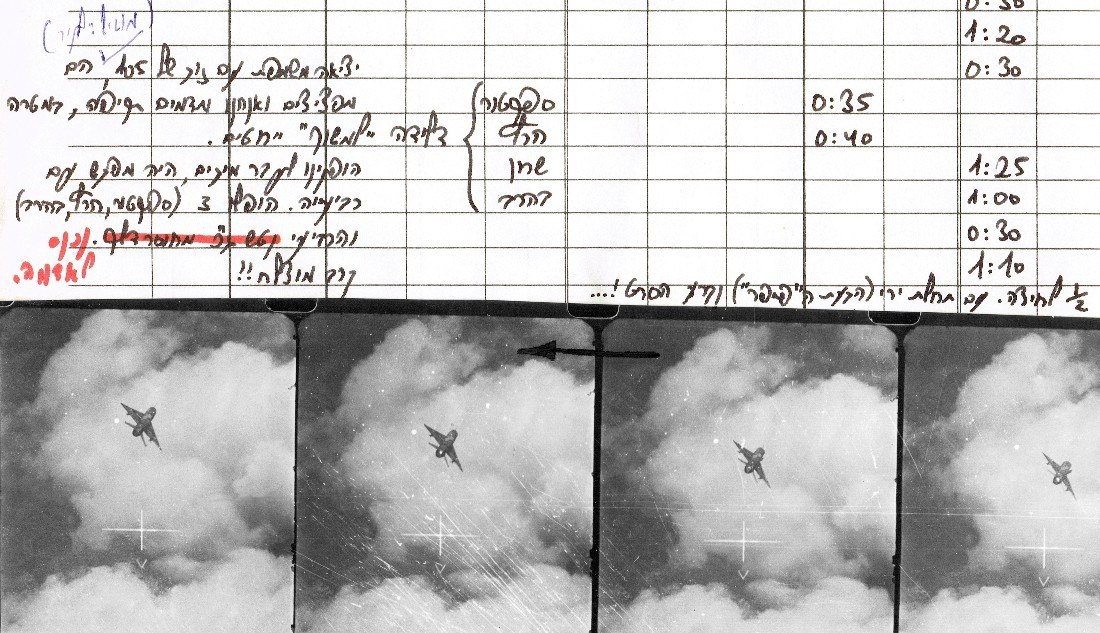
\includegraphics[scale=0.4]{Dolina_0/TXI_-INPzno.jpg}
	%	\label{fig:scipion} % Unique label used for referencing the figure in-text\end{document}
	%	%\addcontentsline{toc}{figure}{Figure \ref{fig:placeholder}} % Uncomment to add the figure to the table of contents%----------------------------------------------------------------------------------------
	\caption{Лётная книжка Йифтаха Спектора (который одержал ту самую спорную пятую победу) Кадры ФКП - мая 1970 (т.е. там не советский МиГ, но всё выглядело примерно так же)}%	CHAPTER 2
\end{figure}

5) Израильтяне крайне неохотно решились на проведение операции - и только после того, как лётчики Настенко (135-й ИАП) начали устраивать засады практически над Каналом. До этого момента связываться с СССР особого желания не было - Израиль не мог выиграть такую войну.

6) Разница между советскими и израильскими пилотами в навыках управления самолётом была не очень большой. В понимании воздушного боя и умении в нём ориентироваться они были просто из разных миров. По израильским меркам, советские пилоты были достаточно "зелеными" и наделали кучу ошибок. Израильтяне тоже не были безошибочны - просто масштаб совсем иной.

7) Со стороны Израиля были лучшие пилоты, которые только могли быть - фактически, комэску каждой из 4 эскадрилий предложили составить список из 4 человек/экипажей для участия в операции - разумеется, каждый начал этот список с себя.

8) Изначальный израильский план был прост - выманить "четверку" советских самолётов и расстрелять их снизу-вверх ракетами "Спэрроу" "Фантомов". Фактически, всё очень быстро пошло не так и пришлось импровизировать.
Советский план - перехватить израильскую пару/звено. Никто не предполагал, что всё получится чуть иначе - в предыдущие 2 месяца в аналогичных ситуациях израильтяне просто уходили на свою сторону канала. Кое-кто в результате расслабился - а зря.


\begin{figure}[h!tb] 
	\centering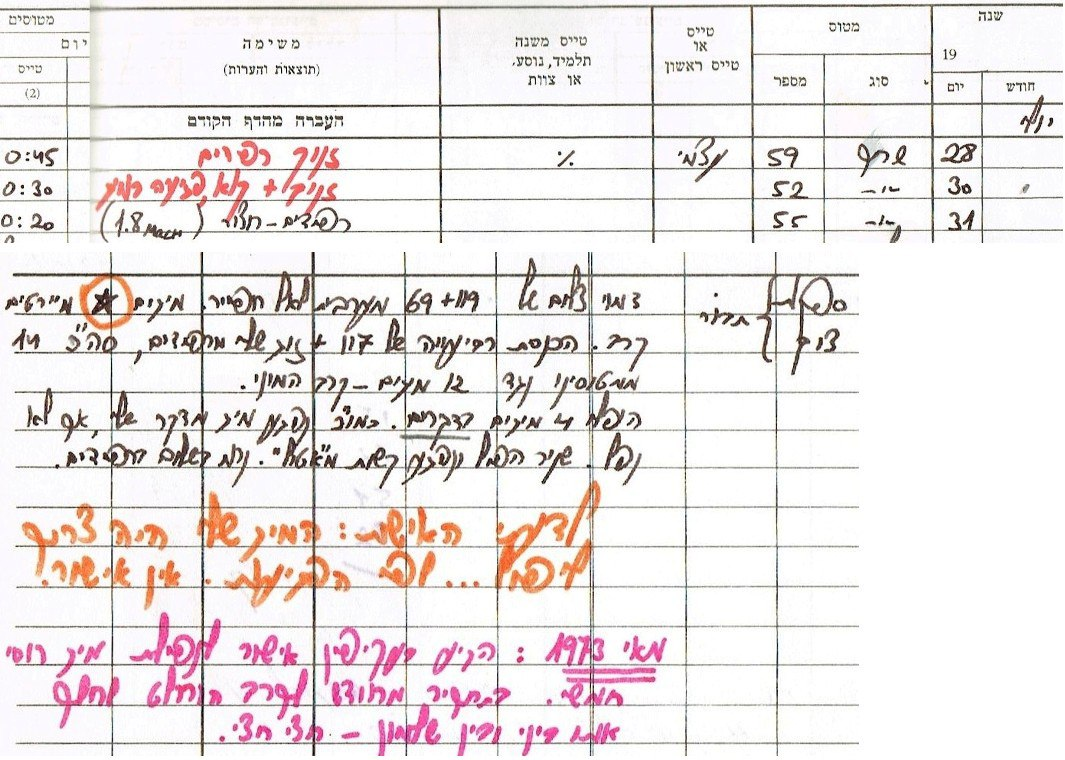
\includegraphics[scale=0.4]{Dolina_0/nYQwdVjlzUE.jpg}
	%	\label{fig:scipion} % Unique label used for referencing the figure in-text\end{document}
	%	%\addcontentsline{toc}{figure}{Figure \ref{fig:placeholder}} % Uncomment to add the figure to the table of contents%----------------------------------------------------------------------------------------
	\caption{фото - с комментарием о "половине" победы, внесенным в 73-м году. Звезду нарисовал сам Спектор. Он вообще был художник в душе и не только.}%	CHAPTER 2
\end{figure}

9) В результате боя, достоверно потеряны 4 МиГ-21, ещё один повреждён. У израильтян, соответственно, один поврежденный Мираж. Насчет пятого самолёта ведутся споры - его Йифтаху Спектору засчитали через три (!) года после боя по данным разведки.




Такие дела.